\documentclass[11pt,a4paper]{article}
\usepackage{fontspec}
\usepackage{setspace}
\usepackage{amsmath,amsfonts,amssymb,amsthm}
\usepackage[margin=1.1in]{geometry}
\usepackage{graphicx}
\usepackage{subfigure}
\usepackage{listings}
\usepackage{booktabs,dcolumn}                     
\usepackage{fancyhdr}
\usepackage{bbm}
\usepackage{multirow}
\usepackage{booktabs}
\usepackage{harvard}
\usepackage{enumerate}
\newcommand{\ra}[1]{\renewcommand{\arraystretch}{#1}}
\DeclareMathOperator{\tr}{tr}
\DeclareMathOperator{\vect}{vec}
\makeatletter
\newcommand*{\rom}[1]{\expandafter\@slowromancap\romannumeral #1@}
\makeatletter

\setstretch{1.4}
\setlength{\headheight}{15pt} 
\graphicspath{{graphs/}}  

\newtheorem{sectheorem}{Example}

 
\begin{document}
\title{Applied Survival Analysis - January 2016\\Solutions to Lab 2: Kaplan-Meier survival estimate}
\date{\vspace{-5ex}}
\author{\vspace{-5ex}}
\maketitle
\begin{enumerate}[(a)]
\item \begin{table}[ht]
\caption{Kaplan-Meier Survival Estimate for the \emph{nhl1} data set.}
% title of Table
\centering
% used for centering table
\begin{tabular}{c c c c c c}
% centered columns (4 columns)
\hline
\hline
 $t^{+}$ & $d_{j}$ & $c_{j}$ & $r_{j}$ 
 &$1-\dfrac{d_{j}}{r_{j}}$&$S(t^{+})$  \\ \hline
     1  & 1 & 0 & 12 & 1-1/12 & 0.917 \\
     2  & 2 & 1 & 11 & 1-2/11 & 0.750 \\
     3  & 1 & 0 & 8  & 1-1/8 & 0.656 \\ 
     5  & 1 & 0 & 7  & 1-1/7 & 0.563 \\
     6  & 1 & 0 & 6  & 1-1/6 & 0.469 \\
     7  & 0 & 1 & 5  & 1-0/5& 0.469 \\ 
     8  & 1 & 0 & 4  & 1-1/4& 0.352 \\ 
    16  & 0 & 1 & 3  & 1-0/3& 0.352 \\ 
    17  & 1 & 0 & 2  & 1-1/2& 0.176 \\ 
    34  & 0 & 1 & 1  & 1-0/1& 0.176 \\
\hline
\end{tabular}
\label{table:1}
\end{table}
Note that $S(t^{+})$ stays the same whenever there is a censored observation only.
Next, we are going to use \verb|R| to obtain the Kaplan-Meier survival estimate. 
So, first we have to import the data into \verb|R|
\begin{footnotesize}
\begin{verbatim}
> # Import data
> nhl1 = read.csv("C:/Applied_Survival_Analysis_Jan2016/lab2/data/nhl1.csv")
> nhl1
   nhltime fail
1        1    1
2        2    1
3        2    1
4        2    0
5        3    1
6        5    1
7        6    1
8        7    0
9        8    1
10      16    0
11      17    1
12      34    0
\end{verbatim}
\end{footnotesize}
The variable \emph{nhltime} denotes the event time while \emph{fail} denotes the failure indicator. Note that, since we are taking censoring into account, the failure indicator will be zero for the censored event times.

We tell \verb|R| that we have survival data through the function \verb|Surv|. The first argument should be the survival time while the second one should be the failure indicator. The formula \verb|Surv(nhltime,fail) ~ 1| means that we are using no covariates.
Then, \verb|survfit|  can be used to get KM estimates.
 Note that by using the option \verb|data = nhl1| we tell \verb|R| where to look for the variables involved in the formula. Add \verb|censored = T| in the \verb|summary| function if you would like to include the censoring times in the output. 
\begin{footnotesize}
\begin{verbatim}
> # KM estimates
> library(survival)
> nhl.fit = survfit(Surv(nhltime,fail) ~ 1,data = nhl1)
> 
> # Add censored = T to include censored event times
> summary(nhl.fit,censored = T)
Call: survfit(formula = Surv(nhltime, fail) ~ 1, data = nhl1)

 time n.risk n.event survival std.err lower 95% CI upper 95% CI
    1     12       1    0.917  0.0798       0.7729        1.000
    2     11       2    0.750  0.1250       0.5410        1.000
    3      8       1    0.656  0.1402       0.4318        0.997
    5      7       1    0.562  0.1482       0.3356        0.943
    6      6       1    0.469  0.1503       0.2501        0.879
    7      5       0    0.469  0.1503       0.2501        0.879
    8      4       1    0.352  0.1517       0.1509        0.819
   16      3       0    0.352  0.1517       0.1509        0.819
   17      2       1    0.176  0.1456       0.0347        0.891
   34      1       0    0.176  0.1456       0.0347        0.891
\end{verbatim}
\end{footnotesize}  
\textbf{Optional:} An object created by \verb|survfit| always contains the number of failures and the number at risk for each time point. Taking advantage of that:
\begin{footnotesize}
\begin{verbatim}
> # (a) OPTIONAL
> km = data.frame(t = nhl.fit$time, dj = nhl.fit$n.event,rj = nhl.fit$n.risk)
> km
    t dj rj
1   1  1 12
2   2  2 11
3   3  1  8
4   5  1  7
5   6  1  6
6   7  0  5
7   8  1  4
8  16  0  3
9  17  1  2
10 34  0  1
> 
> km$lambda.hat = km$dj/km$rj
> km$surv = cumprod(1-km$lambda.hat)
> km
    t dj rj lambda.hat      surv
1   1  1 12 0.08333333 0.9166667
2   2  2 11 0.18181818 0.7500000
3   3  1  8 0.12500000 0.6562500
4   5  1  7 0.14285714 0.5625000
5   6  1  6 0.16666667 0.4687500
6   7  0  5 0.00000000 0.4687500
7   8  1  4 0.25000000 0.3515625
8  16  0  3 0.00000000 0.3515625
9  17  1  2 0.50000000 0.1757812
10 34  0  1 0.00000000 0.1757812
\end{verbatim}
\end{footnotesize}
which is exactly the same with the results from \verb|survfit|.
\item \textbf{Greenwood’s formula:} 
$Var[\hat{S}(t)]=\hat{S}(t)^2\sum_{j:\tau_{j}<t}\dfrac{d_{j}}{(r_{j}-d_{j})r_{j}}$, but since we're evaluating at $t^{+}$, i.e. just after $t$, we have to calculate 
\begin{align}
Var[\hat{S}(t^+)]=\hat{S}(t^+)^2\sum_{j:\tau_{j}\leq t}\dfrac{d_{j}}{(r_{j}-d_{j})r_{j}}\nonumber.
\end{align}
At $t=1$: $Var[\hat{S}(t^+)]=0.917^2\dfrac{1}{11\times12}\Rightarrow
se =\sqrt{Var[\hat{S}(t^+)]} =0.0798$\\
At $t=3$: $Var[\hat{S}(t^+)]=0.656^2\left(\dfrac{1}{11\times12}
+\dfrac{2}{9\times11}+\dfrac{1}{7\times8}\right)\Rightarrow
se =\sqrt{Var[\hat{S}(t^+)]} =0.1402$.\\
The 95\% CIs using the \emph{log-log} approach are calculated through the formula
\begin{align}
[\hat{S}(t^+)^{e^{A}},\hat{S}(t^+)^{e^{-A}}],\nonumber
\end{align}
where $A = 1.96se(\hat{L}(t^+))$, $\hat{L}(t^+)=\log(-\log(\hat{S}(t^+)))$. On page 37 of today's notes we saw that
\begin{align}
Var[\hat{L}(t^+)]=\dfrac{1}{[\log\hat{S}(t^+)]^2}\sum_{j:\tau_{j}\leq t}\dfrac{d_{j}}{(r_{j}-d_{j})r_{j}} \nonumber
\end{align}
At $t^{+}=1$: $Var[\hat{L}(t^+)]=\dfrac{1}{[\log(0.917)]^2}\dfrac{1}{1\times12}
\Rightarrow A = 1.9606$. Thus, the confidence bounds are
\begin{align}
[0.917^{e^{1.9606}}, 0.917^{e^{-1.9606}}] = [0.5390, 0.9878] \nonumber
\end{align}
Be careful here as \verb|R|, unlike \verb|STATA|, does not use by default the \emph{log-log} approach to calculate the CIs. So, we add the option \verb|conf.type = "log-log"| to tell \verb|R| to use the desired method. Then, we use the \verb|plot| function to produce a graph of KM estimates along with the 95\% confidence bounds.
\begin{footnotesize}
\begin{verbatim}
> # (b) 95%CI using the "log-log" approach
> # Be careful here: the default in R is not the "log-log" approach
> nhl.fit = survfit(Surv(nhltime,fail) ~ 1,data = nhl1,conf.type = "log-log")
> summary(nhl.fit,censored = T)
Call: survfit(formula = Surv(nhltime, fail) ~ 1, data = nhl1, conf.type = "log-log")

 time n.risk n.event survival std.err lower 95% CI upper 95% CI
    1     12       1    0.917  0.0798       0.5390        0.988
    2     11       2    0.750  0.1250       0.4084        0.912
    3      8       1    0.656  0.1402       0.3204        0.856
    5      7       1    0.562  0.1482       0.2437        0.791
    6      6       1    0.469  0.1503       0.1762        0.718
    7      5       0    0.469  0.1503       0.1762        0.718
    8      4       1    0.352  0.1517       0.0956        0.628
   16      3       0    0.352  0.1517       0.0956        0.628
   17      2       1    0.176  0.1456       0.0120        0.505
   34      1       0    0.176  0.1456       0.0120        0.505
> 
> setwd("C:/Applied_Survival_Analysis_Jan2016/lab2/graphs")
> 
> pdf('lab2KmSurv.pdf',width = 6,height = 6)
> plot(nhl.fit,main = "Bone Marrow Transplant for Non-Hodgkin's Lymphoma",
+      ylab = "Survival Probability",xlab = "Time to Death or Relapse (months)")
> dev.off()
\end{verbatim}
\end{footnotesize}
The \emph{log-log} approach seems the most appropriate method as it ensures that the bounds fall into the right range (i.e., from 0 to 1). You are strongly advised to use the \emph{log-log} method, especially when the sample size is small.
If you would like to produce the CIs on your own, just type the following
\begin{footnotesize}
\begin{verbatim}
> # 95%CI using our code
> A = qnorm(0.975)*sqrt( cumsum( km$dj/((km$rj-km$dj)*km$rj) )/log(km$surv)^2 )
> km$lower = km$surv^exp(A)
> km$upper = km$surv^exp(-A)
> round(km,4)
    t dj rj lambda.hat   surv  lower  upper
1   1  1 12     0.0833 0.9167 0.5390 0.9878
2   2  2 11     0.1818 0.7500 0.4084 0.9117
3   3  1  8     0.1250 0.6562 0.3204 0.8557
4   5  1  7     0.1429 0.5625 0.2437 0.7910
5   6  1  6     0.1667 0.4688 0.1762 0.7185
6   7  0  5     0.0000 0.4688 0.1762 0.7185
7   8  1  4     0.2500 0.3516 0.0956 0.6278
8  16  0  3     0.0000 0.3516 0.0956 0.6278
9  17  1  2     0.5000 0.1758 0.0120 0.5049
10 34  0  1     0.0000 0.1758 0.0120 0.5049
\end{verbatim}
\end{footnotesize}
\begin{figure}[htbp]
	\centering
		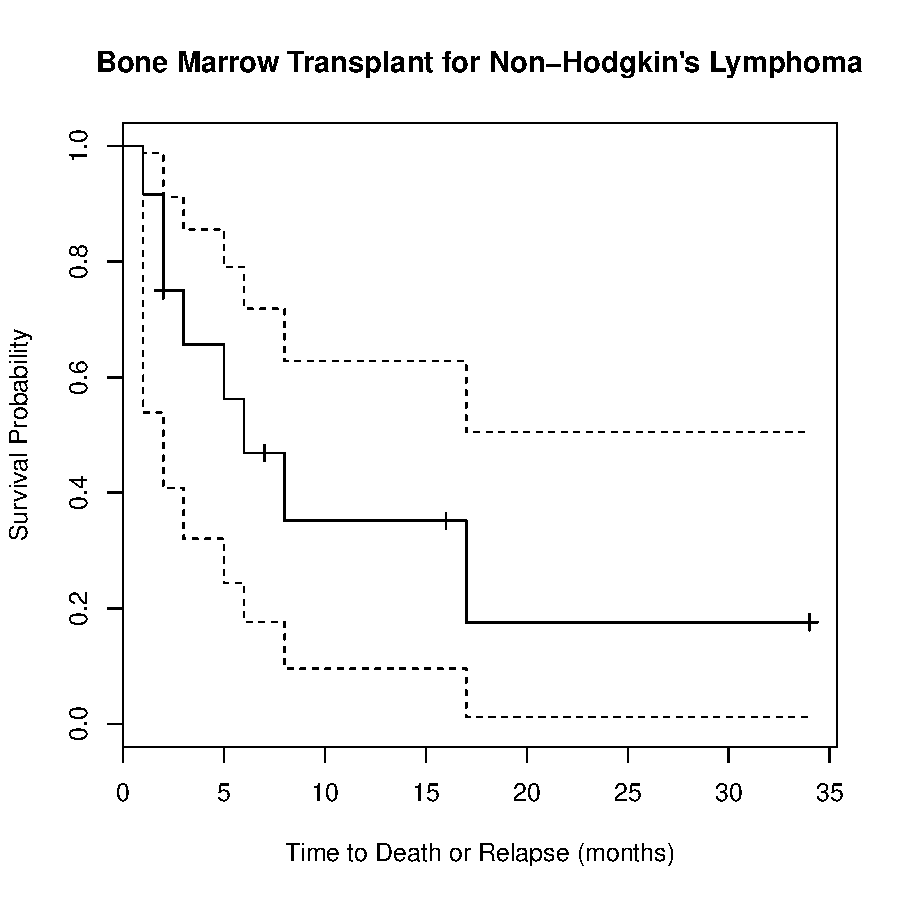
\includegraphics[scale=0.9]{lab2KmSurv.pdf}
		%\rule{35em}{0.5pt}
	\caption{Estimated survival probability for 12 patients
with non-Hodgkin’s lymphoma.}
	\label{figure1}
\end{figure}
\item \textbf{Median:} The smallest time, $\tau$, such that $\hat{S}(\tau^+)\leq 0.5$. Since $\hat{S}(6)=0.4688$, the median survival time is 6 \\
\textbf{Lower quartile (25\%):} The smallest time, $LQ$, such that $\hat{S}(LQ^+)\leq 0.75$. Since $\hat{S}(2)=0.7500$, the the estimated 25\%-ile survival time is 2 \\
\textbf{Upper quartile (75\%):} The smallest time, $UQ$, such that $\hat{S}(UQ^+)\leq 0.25$. Since $\hat{S}(17)=0.1758$, the estimated 75\%-ile survival time is 17.
To get the quartiles in \verb|R|, use the \verb|quantile| function
\begin{footnotesize}
\begin{verbatim}
> # (c): Median survival time, lower and upper quartile
> quantile(nhl.fit,probs = c(0.25,0.5,0.75),conf.int = F)
  25   50   75 
 2.5  6.0 17.0
\end{verbatim}
\end{footnotesize}
As it was mentioned during the previous lab, \verb|R| uses some different algorithm to determine the quartiles.
\item It seems that there is no direct way to get the Nelson-Aalen estimator of the cumulative hazard function in \verb|R|. To do it, we have to use the \verb|coxph| function. You don't need to focus on Cox Regression at this stage. We are going to discuss the Cox regression model a lot soon. Just keep an eye on the following syntax:
\begin{footnotesize}
\begin{verbatim}
> # (d): Nelson-Aalen estimator of the cumulative hazard function
> nhl.na = basehaz(coxph(Surv(nhltime,fail) ~ 1,data = nhl1,ties = "breslow"))
> nhl.na
       hazard time
1  0.08333333    1
2  0.26515152    2
3  0.39015152    3
4  0.53300866    5
5  0.69967532    6
6  0.69967532    7
7  0.94967532    8
8  0.94967532   16
9  1.44967532   17
10 1.44967532   34
> 
> # nhl.na is a data frame with the Nelson-Aalen estimator and the survival times
> # Be aware of the following syntax of the plot function
> pdf('lab2NA.pdf',width = 6,height = 6)
> plot(hazard ~ time,data = nhl.na, type = "b",
+      main = "Bone Marrow Transplant for Non-Hodgkin's Lymphoma",
+      xlab = "Time to Death or Relapse (months)",xlim = c(0,40),ylim = c(0,1.5),
+      ylab = "Nelson-Aalen Cumulative Hazard")
> dev.off()
\end{verbatim}
\end{footnotesize}
An exponential model is only appropriate when the hazard function is constant over time, which 
means that we should expect a straight line in the graph below. In the beginning it seems 
like a straight line but then it curves, so it does not seem likely that an exponential 
distribution would fit these data well. However, since we have only 12 observations, it's hard to tell.
\begin{figure}[htbp]
	\centering
		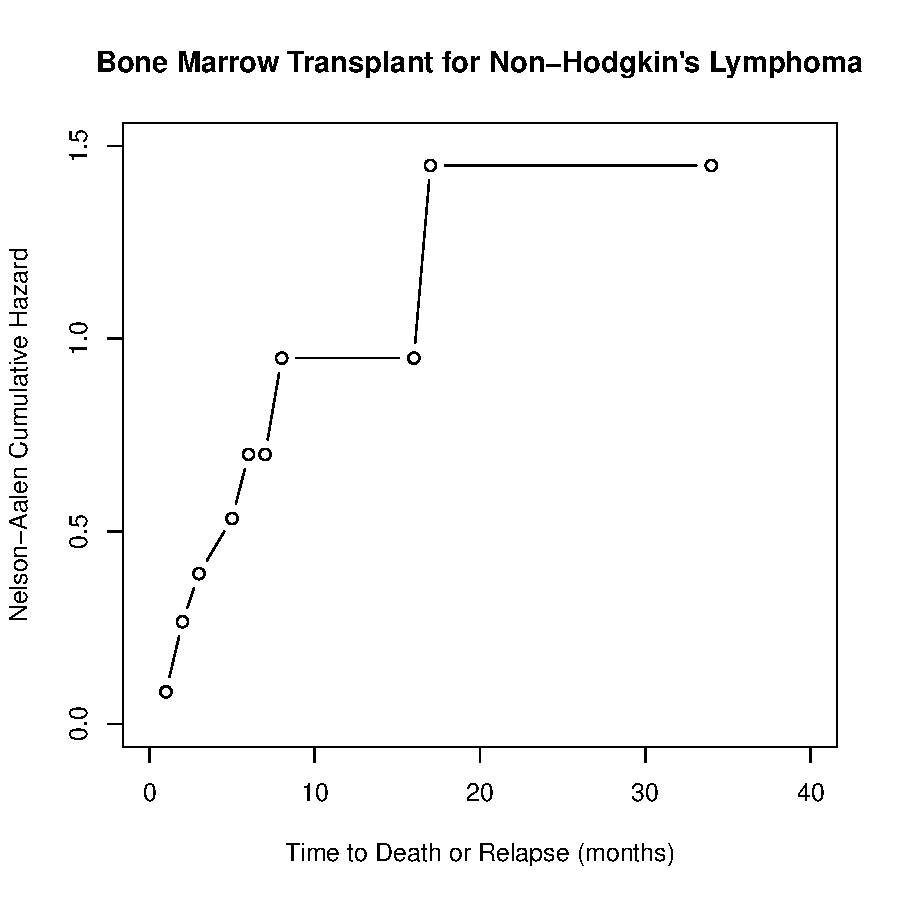
\includegraphics[scale=0.9]{lab2NA.pdf}
		%\rule{35em}{0.5pt}
	\caption{Cumulative hazard function for 12 patients
with non-Hodgkin’s lymphoma.}
	\label{figure2}
\end{figure}
\item We first import the data into \verb|R| and take a look at the dataset. Note that we keep only "treated" nursing homes at this stage
\begin{spacing}{1.2}
\begin{footnotesize}
\begin{verbatim}
> # Import the nurshome data set
> # see lecture 1 for a description of the data
> nurshome = read.csv("C:/Applied_Survival_Analysis_Jan2016/lab2/data/nurshome.csv")
> 
> # Keep only treated 
> nurshome = nurshome[nurshome$rx == 1,]
> head(nurshome)
   los age rx gender married health fail
1  665  83  1      0       0      4    1
3    7  92  1      0       0      4    1
5  153  74  1      1       0      3    1
8   56  84  1      0       0      5    1
9   56  83  1      0       0      3    1
12 162  78  1      1       0      2    1
\end{verbatim}
\end{footnotesize}
\end{spacing}
The \verb|floor(x)| function returns the largest integer not greater than \verb|x|. Thus, to group the length of stay into 100-day intervals, we have to divide it by 100 first.
\begin{spacing}{1.2}
\begin{footnotesize}
\begin{verbatim}
> # Group length of stay into 100-day intervals
> los100 = floor(nurshome$los/100)
\end{verbatim}
\end{footnotesize}
\end{spacing}
In order to be able to use the function \verb|lifetab|, we need to create a couple of variables, mainly the number of censored at each interval and the number of events at each interval. Thus, we need to create grouped data.

Let's try to get the number of events at each interval. Although we could have used \verb|table(los100[nurshome$fail==1])|, we preferred 
\begin{spacing}{1.2}
\begin{footnotesize}
\begin{verbatim}
> # Number of subjects who experienced the event during each interval
> died = tapply(nurshome$fail,los100,sum)
\end{verbatim}
\end{footnotesize}
\end{spacing} 
since
\begin{spacing}{1.2}
\begin{footnotesize}
\begin{verbatim}
> # Why not type table(los100[nurshome$fail==1]) ???
> # They're supposed to be the same! See
> died
  0   1   2   3   4   5   6   7   8   9  10 
328  86  65  38  32  13  13  10   4   4   0 
> table(los100[nurshome$fail==1]) # There is no category for los100 = 10

  0   1   2   3   4   5   6   7   8   9 
328  86  65  38  32  13  13  10   4   4 
\end{verbatim}
\end{footnotesize}
\end{spacing}
that is, typing \verb|table(los100[nurshome$fail==1])| we get no answer for \emph{los100=10}. Note that \verb|tapply| is an extremely useful function in \verb|R|. In this context, it gives us the sum of \emph{nurshome\$fail} for each category of \emph{los100}, i.e. the number of failures for each interval.

Now we'd like to produce the number of censorings at each interval. This is just the total number of times (both censored and uncensored) minus the number of failures.
\begin{spacing}{1.2}
\begin{footnotesize}
\begin{verbatim}
> # Frequency table of length of stay grouped into 100-day intervals
> total = table(los100)
> 
> # Number of censorings at each interval
> censor = total - died
\end{verbatim}
\end{footnotesize}
\end{spacing}
Then after examining \verb|?lifetab|, to obtain the lifetable estimator we need the following code (more in class if needed)
\begin{spacing}{1.2}
\begin{footnotesize}
\begin{verbatim}
> LT.treated = data.frame(LOS100 = unique(los100), died = c(died), censored = c(censor))
> 
> #los100 must have one more length than everyone else
> los100 = sort(LT.treated$LOS100)
> lt = length(los100)
> los100[lt+1] = NA
> 
> # Life table for the angina example
> library(KMsurv)
Warning message:
package ‘KMsurv’ was built under R version 3.1.3 
> nursLT = lifetab(los100, sum(total), LT.treated$censored, LT.treated$died)
> nursLT[,-c(8:10)]
      nsubs nlost nrisk nevent      surv         pdf     hazard
0-1     710     0 710.0    328 1.0000000 0.461971831 0.60073260
1-2     382     0 382.0     86 0.5380282 0.121126761 0.25368732
2-3     296     0 296.0     65 0.4169014 0.091549296 0.24667932
3-4     231     0 231.0     38 0.3253521 0.053521127 0.17924528
4-5     193     1 192.5     32 0.2718310 0.045187489 0.18130312
5-6     160     0 160.0     13 0.2266435 0.018414784 0.08469055
6-7     147     0 147.0     13 0.2082287 0.018414784 0.09252669
7-8     134    30 119.0     10 0.1898139 0.015950750 0.08771930
8-9      94    29  79.5      4 0.1738632 0.008747833 0.05161290
9-10     61    30  46.0      4 0.1651153 0.014357856 0.09090909
10-NA    27    27  13.5      0 0.1507575          NA         NA
\end{verbatim}
\end{footnotesize}
\end{spacing}
Keep in mind that there is no reason to apply the lifetable estimator to such data since they are not actually grouped! We gave the previous approach just for reference. If you would like to produce a graph with the survival and hazard functions predicted by the lifetable estimator use
\begin{spacing}{1.2}
\begin{footnotesize}
\begin{verbatim}
> setwd("C:/Applied_Survival_Analysis_Jan2016/lab2/graphs")
> 
> #Plot of the survival
> pdf("nhact_surv.pdf",height = 5.5,width = 5.5)
> plot(los100[-(lt+1)],nursLT[,5], type="s", 
+      ylab="Survival", xlab="LOS (100-day intervals)")
> dev.off()
RStudioGD 
        2 
> 
> #Plot of the hazard
> pdf("nhact_haz.pdf",height = 5.5, width = 5.5)
> plot(los100[-(lt+1)],nursLT[,7], type="s", 
+      ylab="Hazard", xlab="LOS (100-day intervals)")
> dev.off()
RStudioGD 
        2 
\end{verbatim}
\end{footnotesize}
\end{spacing}

\begin{figure}[htbp]
	\centering
		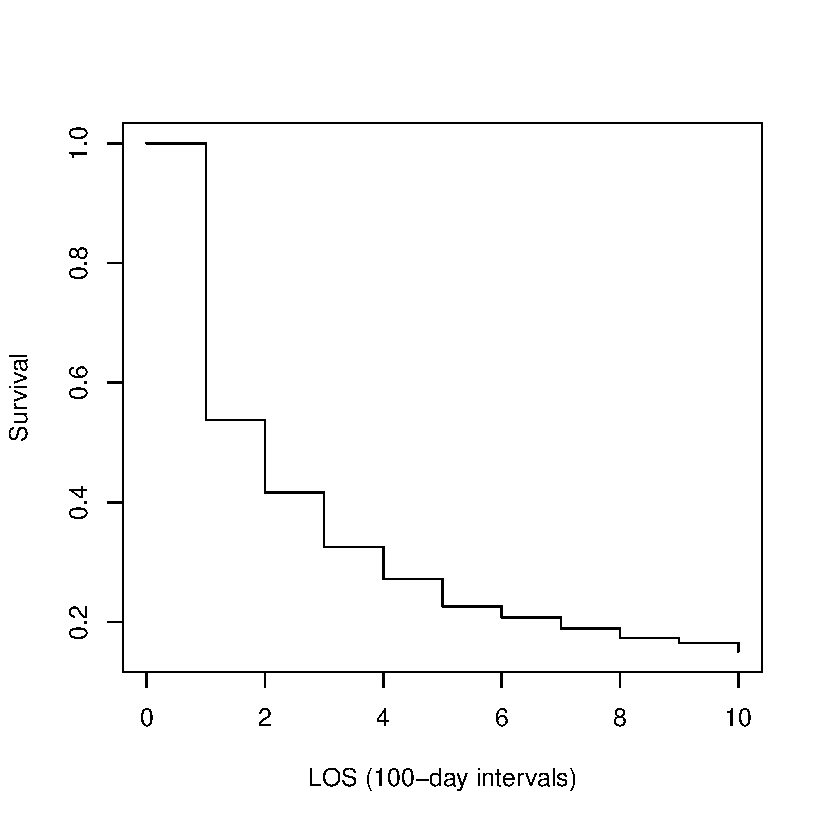
\includegraphics[scale=0.9]{nhact_surv.pdf}
		%\rule{35em}{0.5pt}
	\caption{Estimated survival function in treated nursing homes.}
	\label{figure3}
\end{figure}

\begin{figure}[htbp]
	\centering
		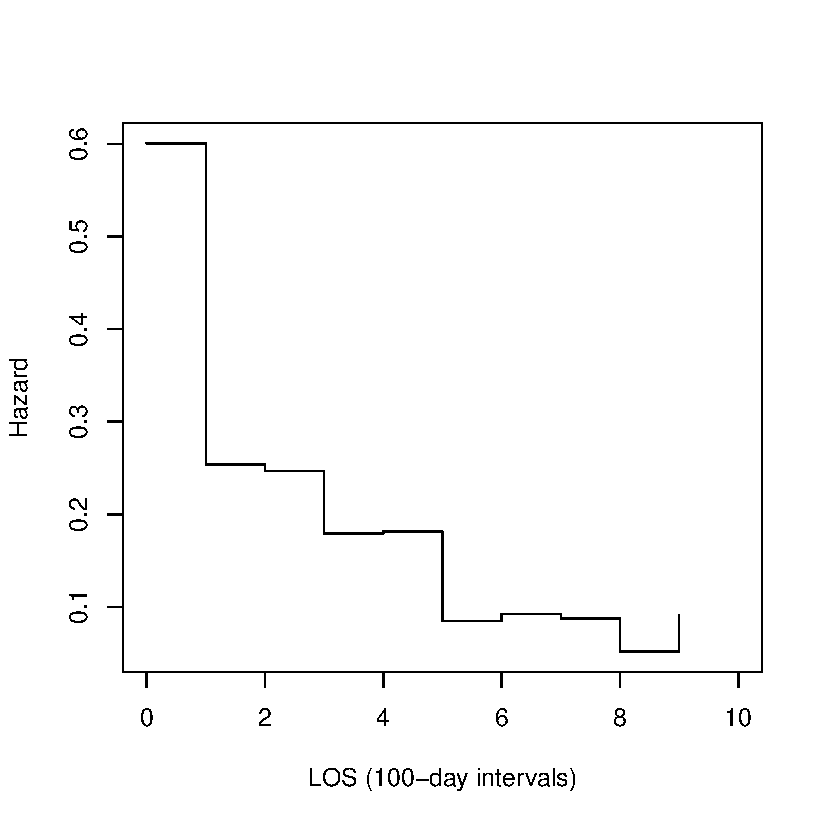
\includegraphics[scale=0.9]{nhact_haz.pdf}
		%\rule{35em}{0.5pt}
	\caption{Estimated hazard function in treated nursing homes.}
	\label{figure4}
\end{figure}
\newpage    
\item \textbf{Optional:} We first construct the \verb|R| function to be used for obtaining the KM estimates
\begin{footnotesize}
\begin{verbatim}
# (f): R function to compute Kaplan-Meier survival estimates
KM = function(surv,delta)
{
  # surv: vector of survival times
  # delta: vector of failure indicator
  data = data.frame(time = surv,fail = delta)
  
  # Sort the dataset with respect to time
  # Pay special attention to this
  data = data[order(data$time),]
  
  time = data$time
  fail = data$fail
  
  # Distinct failure times
  dist.times = unique(time[fail==1])
  K = length(dist.times)
  
  # Number of events for each failure time
  dj = table(time[fail==1])
  
  # Number at risk for each failure time
  # We present a simple but not computationally efficient way to find it
  rj = rep(NA,K)
  
  for (i in 1:K)
  {
    rj[i] = sum(time >= dist.times[i])
  }
  
  # Hazard estimates
  lambda.hat = dj/rj
  
  # Km estimates
  surv.hat = cumprod(1 - lambda.hat)
  names(surv.hat) = NULL
  
  # Output
  out = data.frame(time = dist.times, survival = surv.hat)
  
  return(round(out,4))
}
\end{verbatim}
\end{footnotesize}
Simulating the data
\begin{footnotesize}
\begin{verbatim}
> # We use seed for reproducibility
> set.seed(2)
> 
> n = 30
> # Simulate the (uncensored) survival times
> surv = exp(rnorm(n, mean = - 1, sd = 0.5))
> 
> # Simulate the censoring timess
> cens = rexp(n, rate = 2)
> 
> # Failure indicator
> # 1, if survival time < censoring time
> # 0, if survival time >= censoring time
> delta = 1*(surv < cens)
> 
> # Observed survival time
> # time = surv if surv < cens
> # time = cens if surv >= cens
> time = pmin(surv,cens)
> 
> # Using survfit
> data = data.frame(time = time, fail = delta)
> fit = survfit( Surv(time,fail) ~ 1, data = data)
> summary(fit)
Call: survfit(formula = Surv(time, fail) ~ 1, data = data)

  time n.risk n.event survival std.err lower 95% CI upper 95% CI
 0.108     27       1    0.963  0.0363       0.8943        1.000
 0.116     25       1    0.924  0.0514       0.8290        1.000
 0.202     20       1    0.878  0.0664       0.7572        1.000
 0.209     19       1    0.832  0.0774       0.6934        0.998
 0.235     17       1    0.783  0.0869       0.6299        0.973
 0.302     15       1    0.731  0.0955       0.5657        0.944
 0.326     14       1    0.679  0.1020       0.5055        0.911
 0.353     13       1    0.626  0.1067       0.4487        0.875
 0.369     12       1    0.574  0.1098       0.3948        0.835
 0.393     11       1    0.522  0.1115       0.3434        0.794
 0.425      9       1    0.464  0.1132       0.2876        0.749
 0.457      8       1    0.406  0.1130       0.2354        0.700
 0.524      7       1    0.348  0.1107       0.1866        0.649
 0.547      6       1    0.290  0.1064       0.1413        0.595
 0.571      5       1    0.232  0.0997       0.1000        0.539
 0.814      4       1    0.174  0.0901       0.0631        0.480
 0.897      3       1    0.116  0.0765       0.0319        0.422
 0.978      1       1    0.000     NaN           NA           NA
> 
> # Our function
> KM(time,delta)
     time survival
1  0.1080   0.9630
2  0.1158   0.9244
3  0.2019   0.8782
4  0.2090   0.8320
5  0.2349   0.7831
6  0.3023   0.7309
7  0.3263   0.6787
8  0.3534   0.6264
9  0.3688   0.5742
10 0.3931   0.5220
11 0.4252   0.4640
12 0.4566   0.4060
13 0.5241   0.3480
14 0.5467   0.2900
15 0.5708   0.2320
16 0.8145   0.1740
17 0.8968   0.1160
18 0.9776   0.0000
\end{verbatim}
\end{footnotesize}
We can see that the results from both functions are exactly the same.
\end{enumerate}



\end{document}